%% -*- coding: utf-8 -*-
\documentclass[12pt,pagesize,paper=192mm:108mm]{scrbook} 
%1920x1080 1280x720
\areaset[current]{192mm}{108mm}
\usepackage{calc}
\usepackage[T2A]{fontenc}
\usepackage[utf8]{inputenc}
\usepackage[english,russian]{babel}
\usepackage{microtype}
\usepackage{misccorr}
\usepackage{cmap}
%\usepackage[unicode=true]{hyperref}
\usepackage{graphicx}
\usepackage{amssymb}
\usepackage{amsmath}
%\usepackage{srcltx}
\usepackage{textcomp}
\usepackage{xspace}
%научные символы и смайлики \smiley \frownie
\usepackage{wasysym}
\usepackage{ccicons}
\DeclareMathOperator{\Tr}{Tr}
%перенос формул в тексте
\newcommand*{\hm}[1]{#1\nobreak\discretionary{}%
  {\hbox{$\mathsurround=0pt #1$}}{}}
\renewcommand{\epsilon}{\varepsilon}
\begin{document}
\begin{titlepage}
  \vspace*{-0.5em}
  \begin{center}    
    \hspace*{3em}
    \begin{minipage}[t]{3em}
      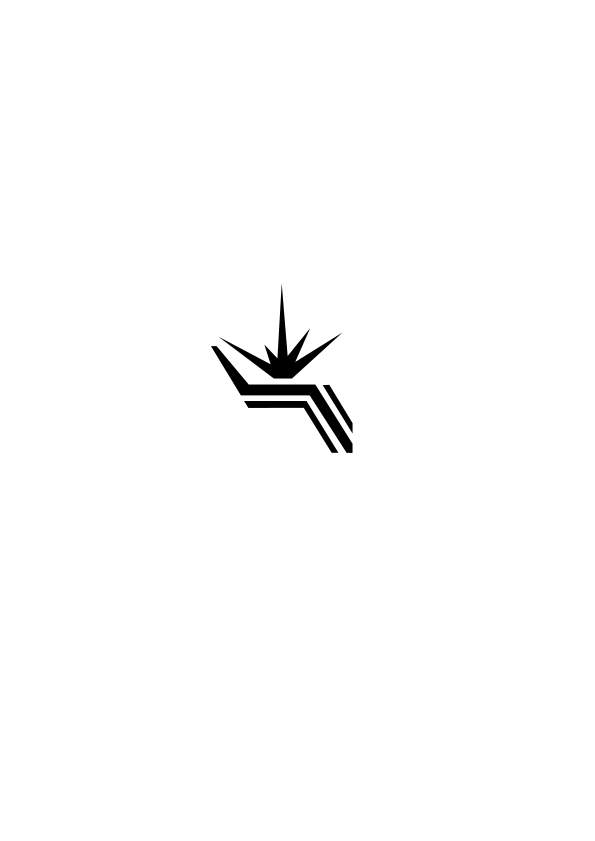
\includegraphics[width=\textwidth]{../BINP-logo}
    \end{minipage}\hfill
    \begin{minipage}{0.23\linewidth}
    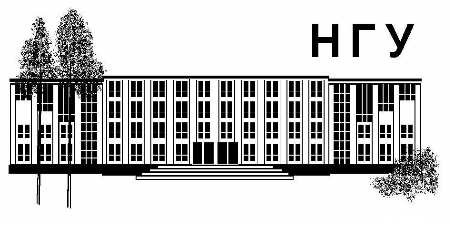
\includegraphics[width=\textwidth]{../NSU-logo}
    \end{minipage}
    \hfill
    \hspace*{6em}

    Кафедра теоретической физики физического факультета НГУ
    \medskip

    \Large
    Резниченко А.\,В.
    \bigskip

    \huge
    \textbf{Квантовая электродинамика}
    \bigskip

    \Large
    Семинар № 1
    \vfill

    \normalsize
    \vfill

    \normalsize \ccbysa\hspace{0.5em}  Новосибирск 2015
  \end{center}
\end{titlepage}
\newpage

\vspace*{-1em}
\begin{center}
\vfill
  \begin{minipage}{0.65\linewidth}
    Алгебра $\gamma$"=матриц.  Краткое введение: алгебра матриц
    $\gamma^{\mu}$, матрица $\gamma^5$, тензоры
    $\epsilon^{\mu\nu\alpha\beta}$ и $g^{\mu\nu}$ в группе Лоренца,
    $\gamma$"=матрицы в D измерениях.
    Задача вычисления сверток $\gamma^{\mu}\Gamma\gamma_{\mu}$ для
    разных матриц $\Gamma$ в~размерности $D=4+2\epsilon$.
    Задача вычисления различных следов с~$\gamma$"=матрицами:
    рекуррентное выражение для следа $\Tr[\gamma^{\mu_1}\ldots
    \gamma^{\mu_N}]$ и аналогия с теоремой Вика для фермионных
    операторов (структура спариваний в теореме Вика, полное число
    спариваний). Простейшие следы $\Tr[\gamma^{\mu}\gamma^{\nu}]$,
    $\Tr[\gamma^{\mu}\gamma^{\nu}\,\gamma^{\alpha}\gamma^{\beta}]$,
    $\Tr[\gamma^5\gamma^{\mu}\gamma^{\nu}\,\gamma^{\alpha}\gamma^{\beta}]$,
    нулевые следы и проч. Пакет FeynCalc.
    \smallskip

    Задача: вывод соотношения полноты для~$\gamma$"=матриц при
    $D=4$. Преобразование спиноров при лоренцевских преобразованиях,
    генераторы преобразований (напоминание). Пример: разложение
    произведения $\gamma^{\mu}\gamma^{\alpha}\gamma^{\nu}$ по базису
    $\gamma$"=матриц: $\gamma^{\mu}\gamma^{\alpha}\gamma^{\nu}=
    g^{\mu\alpha}\gamma^{\nu} + g^{\nu\alpha}\gamma^{\mu}\hm{-}
    g^{\mu\nu}\gamma^{\alpha}+ i \epsilon^{\mu\alpha\nu\beta}\gamma_{\beta}
    \gamma^5$.  
    Преобразования для~$\gamma$"=матриц при эрмитовом и комплексном
    сопряжении, а также при~транспонировании.
  \end{minipage}
  \vfill

  % \normalsize \ccbysa\hspace{0.5em} Новосибирск 2013
\end{center}
\end{document}
